\subsection{Results from interviews}
There are several reasons why the current recruitment process needs to be optimized.

\begin{enumerate}
\item The main frustrations in the IT-department are that some recruitments occur with very short notice, and that data occasionally is incomplete.\\
(Appendix \completeref{app:peter} lines \lineref{peter_datamangel}, \lineref{peter_frustration1}, \lineref{peter_frustration2}, and \lineref{peter_frustration3}).
\begin{itemize}
\item The incomplete data for the IT department occurs with recruitments from OMT, while the short notices mainly are rooted in the recruitment of subcontractors in OMT.\\
(Appendix \quoteref{app:peter}{peter_short_notice}).
\item Part of the problem with incomplete data is that the recruiters are not aware of exactly what information is needed in order to set a new employee up correctly.\\
(Appendix \quoteref{app:jytte}{jytte_stamdata}).
\item Valcon employees have a notion that the IT department should be able to handle everything with short notice. Not all IT employees share this opinion.\\
(Appendix \quoteref{app:peter}{peter_klare_IT_bare} and \quoteref{app:hanne_interview}{hanne_snakker_om_IT}).
\end{itemize}

We think that some of the frustration stems from IT not having a standard process for when data is incomplete.

\item The main frustration in Accounting is that it is difficult to get an overview, as employee data is managed in many different systems, and that data is incomplete.\\
(Appendix \quoteref{app:lisbeth}{lisbeth_overblik}).
\begin{itemize}
\item Each employee in the recruitment process maintains their data on the new employees in individual spreadsheets.\\
(Appendix \quoteref{app:lisbeth}{lisbeth_ark}).
\end{itemize}

This is problematic, as responsibility of the current process is difficult to pass on to another accountant.

\item A lot of time is spent communicating information back and forth between Accounting and Recruitment. \\
(Appendix \quoteref{app:lisbeth}{lisbeth_vende_tilbage}).
\begin{itemize}
\item Similarly time is spent communicating information to the IT-department.\\
(Appendix \quoteref{app:lisbeth}{lisbeth_IT}).
\item Accounting and IT want communication to be more standardized. Recruitment finds this problematic because data may be missing at the time of recruitment.\\
(Appendix \quoteref{app:lisbeth}{lisbeth_standardiseret_proces}, \quoteref{app:peter}{peter_standardiseret_proces} and \quoteref{app:hanne_interview}{hanne_ikke_standardiseret_proces}).
\item Forcing standardized communication might put additional pressure on the consultant/manager in charge of the recruitment, which should be avoided.\\
(Source: appendix \quoteref{app:hanne_interview}{hanne_standardised}).
\item At OMT requiring standardized communication might be possible.\\
(Source: appendix \quoteref{app:jytte}{jytte_standardised}).
\end{itemize}

With a common system for keeping the information, problems 2. and 3. could be avoided, as everyone could view the data within that system.

\item Time is spent on routine tasks, such as defining new initials.\\
(Appendix \quoteref{app:peter}{peter_initialer}).

This could possibly be automated.

\item Time is wasted waiting for other IT employees, as IT doesn't have standard processes for communication.\\
(Appendix \quoteref{app:emails}{matias_on_structure}).

This is outside our scope, but should be investigated.
\end{enumerate}

A visual representation of the chain of problems can be found in appendix \ref{app:ProblemChain}.
Note from the interviews can be found in appendix \ref{app:interviews}.

\subsection{The numbers}
\todo{Merrild splitter cost/benefit op i to og referer til den første i det her}
\begin{wrapfigure}{r}{0.5\textwidth}
\vspace{-20pt}
\centering
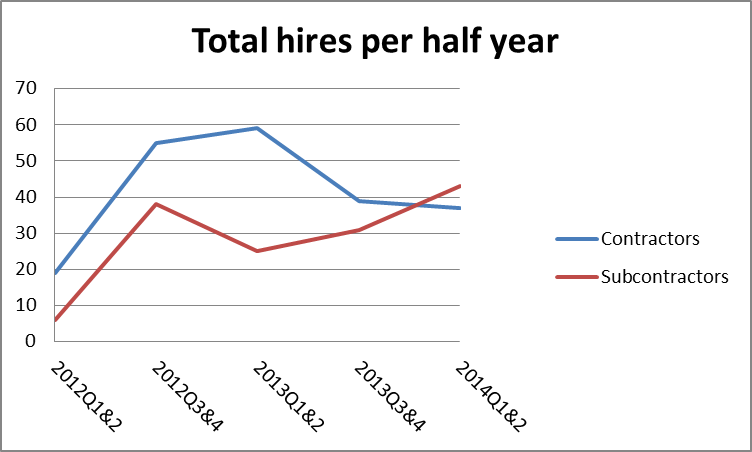
\includegraphics[width=0.45\textwidth]{appendix/total_hires_per_half_year.png}
\label{fig:total_hires_per_half_year}
%\caption{Total number of new hires per half year.}
\end{wrapfigure}
Looking at the number of new hires in Valcon we got an impression of the scope of the problem.
Even though there are some fluctuations there is a trend toward a growth in the number of hires.
This corresponds with the expressed business strategy of growth.
However, the data is not entirely conclusive, as we have only been able to look at the number of new hires within the last 30 months.
A table with all the numbers of new hires can be found in appendix \ref{app:recruitment_data} together with additional graphs.